\documentclass[a4paper,12pt,twoside,openright]{book}

\usepackage[english]{babel}
\usepackage[T1]{fontenc}
\usepackage[utf8]{inputenc}
\usepackage{lmodern}
\usepackage{fancyhdr}
\usepackage{float}
\usepackage{graphicx}
\usepackage{wrapfig}
\usepackage{setspace}

%------------------------------ colors
\usepackage[usenames,dvipsnames,table]{xcolor} % use colors on table and more
\definecolor{333}{RGB}{51, 51, 51} % define custom color
%------------------------------ source code
\usepackage{listings}
\lstset{
  basicstyle=\footnotesize\sffamily,
  commentstyle=\itshape\color{gray},
  captionpos=b,
  frame=shadowbox,
  language=HTML,
  rulesepcolor=\color{333},
  tabsize=2
}
%------------------------------ define Abstract environment, missing in the 'book' class
\newenvironment{abstract}{\cleardoublepage \null \vfill \begin{center}\bfseries\abstractname \end{center}}{\vfill\null}
%------------------------------ active url
\usepackage{url}
\renewcommand{\UrlFont}{\color{black}\small\ttfamily}
\usepackage[colorlinks=true, linkcolor=black, citecolor=black, urlcolor=black]{hyperref} % active ref
%------------------------------ macros
\newcommand{\sectionname}{Section} % define Section ref
\newcommand{\subsectionname}{Sub-section} % define Sub-section ref
\renewcommand*\arraystretch{1.4} % tables padding


\begin{document}
\frontmatter
\begin{titlepage}
	%immagini di intestazione
	\begin{flushleft}
		
\includegraphics[width=0.3\columnwidth]{images/logo_unipd.png}
		\hspace{\fill}
		
\includegraphics[width=0.05\columnwidth]{images/logo_DEI.png}
		\hspace{0.01 cm}
		\begin{minipage}[b][1,8 cm][c]{0.3\columnwidth}
			\textsf{{\color{Sepia}{DIPARTIMENTO\\DI INGEGNERIA\\DELL'INFORMAZIONE}}}
		\end{minipage}
	\end{flushleft}
	
	%titoli vari
	\vfill
	\begin{center}
		\begin{large}
			DEPARTMENT OF INFORMATION ENGINEERING
			\\~\\
			BACHELOR'S DEGREE IN COMPUTER ENGINEERING
			\\~\\~\\
			Fusing vision and inertial measurements for autonomous navigation in narrow channels
			\vfill
			Supervisor: 
			\hfill
			Candidate:
			\\
			Prof. Damiano Varagnolo
			\hfill
			Thomas Sanavia
			\vfill
			ACADEMIC YEAR: 2024/2025
			\\
			Graduation date: -- -- ----
			\vfill
		\end{large}
	\end{center}
	
\end{titlepage}


\cleardoublepage % make left page blank
\thispagestyle{empty} %------------------------------ DEDICA

\null
\vspace{2cm}
\begin{flushright}
A ...
\end{flushright}
\vfill

\begin{quote}
  Quote

  \textit{Author}
\end{quote}
\vfill
\null


\begingroup %------------------------------ CONTENTS
  \makeatletter
  \let\ps@plain\ps@empty
  \makeatother
  \tableofcontents
\endgroup

\begin{abstract} %------------------------------ ABSTRACT
\markboth{}{} % remove header
\thispagestyle{empty}
This thesis addresses the design, development, and validation of an automatic system for detecting roll, pitch, and yaw of an autonomous boat. The main objective is to create a low-cost, low-power, and easily transportable solution capable of accurately determining the boat’s attitude. To achieve this, both computer vision and an onboard inertial sensor will be used. By fusing data from these two sources, a precise estimate of the boat’s attitude will be made available to the entire system. For the computer vision part, two cameras will be used to exploit stereo vision. The attitude estimation will be processed on a Raspberry Pi 5, chosen for its low cost. For this purpose, ArUco Tags—two-dimensional fiducial markers commonly used in robotics and augmented reality for pose estimation—will be employed. Regarding the inertial sensor, the onboard device will provide velocities and accelerations along the three axes. Finally, an extended Kalman filter, which will utilize both inertial and computer vision data, will be applied to reduce drift and improve the accuracy of roll, pitch, and yaw estimation.
\end{abstract}



\mainmatter\doublespace 

\chapter*{Introduction} %------------------------------ INTRODUCTION
\addcontentsline{toc}{chapter}{Introduction}
\thispagestyle{empty}
In recent years, the field of \textbf{autonomous systems} has played an increasingly central role in robotics. All this has also been made possible thanks to solutions such as \textbf{Robot Operating System 2 (ROS2)}, which is one of the platforms for the development of robotic applications. This has been achieved thanks to its modular architecture, support for real-time communication, and its open-source nature, which has made it an excellent choice even for advanced robotic systems.  

This thesis is part of the \textbf{Autodocking project}, focused on the ability of a boat to navigate and dock autonomously. Although the structure and the basic control systems were already in place, a computer vision–based system for autonomous navigation was missing. My contribution was related to the creation of a ROS2 node; more specifically, I dealt with the entire pipeline ranging from image acquisition, attitude estimation, and subsequent sensor fusion with the inertial sensor data. To achieve this, I needed a ROS2 node that handled the acquisition of images from the various cameras installed on the boat and their publication on a topic, so that my algorithm could access them.

% --- Pagina bianca con numero romano
%\cleardoublepage
%\null
%\thispagestyle{plain} % mantiene il numero di pagina
%\addtocounter{page}{1} % opzionale, LaTeX normalmente incrementa automaticamente

\chapter{Introduction}
\thispagestyle{empty}
\section{Autonomous Surface Vehicles: challenges and applications}
Unmanned Surface Vehicles (\textbf{USVs}) are particular surface vessels capable of navigating without the presence of a human crew to maneuver them. They can be \textit{remotely operated} through radio or satellite communication, or be completely \textit{autonomous} and controlled by a computer or artificial intelligence; in this case, they are referred to as \textbf{Autonomous Surface Vehicles (ASVs)}. ASVs aim to make journeys \textit{safer}, \textit{reduce costs}, \textit{increase operational continuity}, and carry out \textit{prolonged missions} in \textit{complex} and even \textit{risky} situations for humans.\\

All this has been made possible thanks to significant technological evolution in \textbf{sensors} (satellite, IMU, cameras, LIDAR, radar, etc.), major developments in \textbf{robotics libraries}, and onboard \textbf{computational power} that is increasingly greater and more affordable. Despite this, the \textbf{marine environment} presents major challenges. For example, the \textit{plane of the sea surface} is not a fixed reference but changes independently of the boat’s movements; the surface creates \textit{reflections} that can interfere with instrumentation; and \textit{wind and waves} can put stability control systems to the test. In the marine context, therefore, \textbf{attitude estimation} (roll, pitch, and yaw) is essential, as it is decisive both for the \textit{success of the journey} and for the \textit{precision required in maneuvers}, such as docking.\\

The main challenges concern \textbf{sensors and algorithms}. The first challenge involves \textbf{navigation with GNSS} (Global Navigation Satellite System), which degrades in proximity to port infrastructures, bridges, or areas with many vertical obstacles, as part of the visible satellites are lost. This problem has been partly mitigated with \textbf{inertial sensors (IMU)}, which, however, suffer from another issue: \textit{drift}. The second challenge is the \textbf{detection of possible obstacles} at sea, such as buoys, debris, or even other vessels, often under conditions of \textit{reduced visibility} or \textit{reflections}. The third challenge is \textbf{control and stability}, made complex by \textit{wave motion} that often causes very rapid variations. The last challenge is the ability to make \textbf{real-time decisions}, including very quick changes dictated by sudden shifts in the operational situation.\\

Despite the criticality of these challenges, ASVs are used in various \textbf{applications}. In the \textbf{industrial field}, they are employed for \textit{infrastructure inspection} or \textit{short-range logistical support}. In \textbf{defense and security}, they are used in \textit{special operations} such as \textit{explosive ordnance disposal}. In the \textbf{environmental field}, they are used for \textit{monitoring environmental parameters} and \textit{collecting meteorological data} over extended time horizons, thereby reducing risks for crews.\\

Within this framework, the present thesis focuses on one main issue: obtaining an \textbf{accurate real-time estimation} of the boat’s attitude. To achieve this, \textbf{computer vision techniques} (stereo vision and ArUco markers), \textbf{inertial measurements} through the IMU, and an \textbf{Extended Kalman Filter} will be used to fuse the data, with the aim of \textit{improving the reliability of the estimation}.

\section{Attitude Estimation: roll, pitch, yaw}

To describe the \textbf{attitude} of a vessel, the orientation of the rigid body with respect to a reference system is used. This is done through the three \textbf{Euler angles}\cite{Euler_angles}: \textit{roll} (rotation on the longitudinal axis), \textit{pitch} (rotation on the transverse axis), and \textit{yaw} (rotation on the vertical axis). These three quantities are \textbf{crucial} as they influence \textbf{stabilization} and \textbf{trajectory control} and are fundamental in \textbf{precision maneuvers}.  

\begin{figure}[ht]
  \centering
  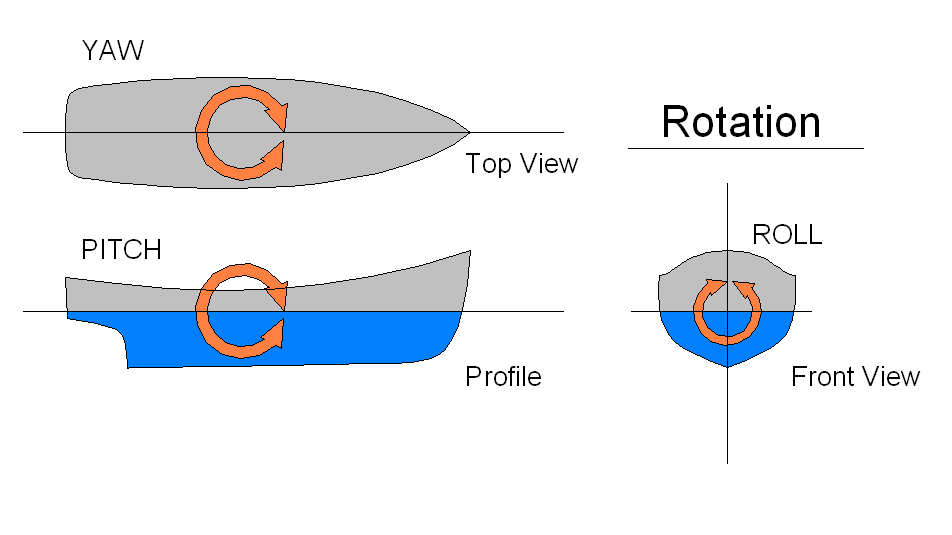
\includegraphics[height=6cm]{images/euler_angles.png}
  \caption{Three rotational degrees of freedom of a ASV}\label{unipd-logo}
\end{figure}


\textbf{Attitude estimation} can be obtained from different sources, each with its own advantages and disadvantages. \textbf{Inertial sensors (IMU)}\cite{IMU_Euler}, through gyroscopes and accelerometers, provide roll and pitch with a \textbf{high update frequency}. However, these estimates are affected by \textit{drift}, caused by the accumulation of errors over time. For yaw, a \textbf{magnetometer} or an \textbf{external observation} is required, as the IMU does not provide a direct measurement of this angle. A \textbf{visual sensor} allows estimating the attitude through \textit{known structures} (e.g., ArUco tags) or through the environment if it allows it (e.g., using the \textit{horizon line}). This latter method is less affected by the drift problem but is highly sensitive to \textbf{environmental conditions} and also has a \textbf{lower update frequency}.  

In the \textbf{marine context}, a robust pipeline is represented by the IMU, which provides a \textbf{high-frequency prediction} and, periodically, through \textbf{computer vision}, a measurement relative to the ArUco marker to reduce error accumulation. Through an \textbf{EKF filter}\cite{EKS_IMU_cv}, the different contributions are integrated in order to obtain a \textbf{coherent estimate} even if the conditions are adverse or if one of the sources fails.  

In summary, \textbf{attitude estimation} for an \textbf{ASV} requires a compromise between the \textbf{speed of the readings} and their \textbf{accuracy}. The \textbf{integration} between \textit{inertial} and \textit{visual} measurements provides a \textbf{reliable estimate} capable of supporting \textbf{autonomous navigation}. Subsequently, the different \textbf{implementation choices} to obtain the attitude estimation of the \textbf{Blue Boat} will be presented.  

\section{Computer Vision for Localization and Attitude Estimation}

Computer vision is an essential source for estimating the attitude of the ASV. 
It provides \textbf{roll}, \textbf{pitch}, and \textbf{yaw} with respect to a known reference, 
namely the \textit{ArUco marker}. In our case, it plays a \textit{complementary role} with respect to the IMU, 
which provides an absolute measurement that is not obtained through temporal integration, 
but is instead sensitive to visual conditions (\textit{reflections, backlighting, fog, etc.}).\\
The goal of this chapter is to outline the principles and choices that allow for reliable 
attitude estimation using a \textbf{stereo camera pair}, leveraging \textit{ArUco markers} 
and a geometric calibration of the two cameras.\\

The pipeline is structured into four main steps:
\begin{itemize}
    \item \textbf{Stereo camera calibration:} estimation of intrinsic parameters and distortions, 
    followed by the calculation of rotation and translation between the two cameras.
    \item \textbf{Marker detection:} ArUco markers enable highly reliable identification, 
    provided they are properly scaled according to the distance and have a sufficient pixel resolution.
    \item \textbf{Attitude estimation:} application of a pose estimation algorithm which, 
    knowing the 2D corners and the 3D points of the pattern, can estimate the values of roll, pitch, and yaw.
    \item \textbf{Measurement validation:} a decision filter determines whether to accept the measurement, 
    discard it, or reduce its influence.
\end{itemize}

Triangulation, made more reliable by \textbf{epipolar rectification}, allows for the estimation of depth around the marker. 
These depth cues are used as additional support to improve the attitude estimation.\\

Finally, temporal and synchronization aspects also play a \textbf{crucial role}. 
Synchronization is \textit{decisive} to avoid disparities and inconsistent triangulations. 
The frame rate and the subsequent update time strongly influence the \textbf{accuracy} of the algorithm’s estimation, 
since excessively low values reduce its quality.\\

This approach, entirely based on stereo vision and ArUco markers, enables precise attitude estimation. 
Its accuracy is determined by the quality of calibrations and the robustness of estimation algorithms, 
but it reaches its maximum effectiveness when \textbf{integrated with IMU data}, 
compensating for the weaknesses of each source.

\section{Fiducial markers and ArUco tags}

The \textbf{ArUco marker} is a square planar pattern with a high-contrast black border and an internal matrix encoding a \textit{unique identifier}. This structure allows for fast localization and recognition of the four corners, providing a stable 2D--3D correspondence for attitude estimation. The use of a single marker reduces environmental and economic requirements. However, relying on just one marker requires greater care in localization, calibration, and validation of the measurements.\\

The recognition pipeline adopts a pair of calibrated cameras. After calibration of the individual cameras and subsequent stereo calibration (\textit{rotation, translation, and epipolar rectification}), the images are acquired and rectified, thus aligning the epipolar lines. The detection of the marker involves several steps:

\begin{enumerate}
    \item Adaptive thresholding
    \item Contour extraction
    \item Quadrilateral selection
    \item ID decoding\\
\end{enumerate}

Knowing the marker size, the attitude is calculated through the \textbf{PnP algorithm (Perspective-n-Point)}, obtaining the rotation and translation of the reference camera frame. If both cameras observe the marker, the two estimates can be fused, or the one with higher quality can be selected.\\

The use of a system based on \textbf{stereo vision} improves disparity estimation in the regions close to the marker and enables \textit{metric triangulation} of depth, enhancing stability compared to a monocular approach. This becomes particularly evident when the marker is very small (i.e., far away) or when it is not perpendicular to the viewing angle, as both conditions reduce perspective information.\\

For each estimate, quality indicators are evaluated: reprojection error, effective presence of the marker (all four corners detected), and the angle between the camera and the marker, penalizing views that are too oblique. Furthermore, a comparison is made between the apparent size of the marker in pixels, in order to identify discrepancies due to triangulation or temporal misalignment. \\

From a practical point of view, the use of a single ArUco marker offers a \textbf{simple and easily reproducible implementation path}: a single print on a rigid surface with a matte finish (to reduce reflections) is sufficient. Under these conditions, a single ArUco marker used in a well-calibrated stereo vision pipeline provides roll, pitch, and yaw measurements while maintaining a \textit{good trade-off between precision and computational demand}.
\chapter{Attitude Estimation with Computer Vision}
\thispagestyle{empty}
\section{Vision Hardware and Experimental Setup}
\begin{table}[h]
    \centering
    \begin{tabular}{|c|c|c|c|}
        \hline
        \textbf{Component} & \textbf{Model/Version} & \textbf{Role} & \textbf{Cost} \\
        \hline
        Raspberry Pi 5 & 8GB RAM & Frame acquisition and attitude computation & 85€ \\
        \hline
        Right Pi Camera & V3 & Capture right frame & 27€ \\
        \hline
        Left Pi Camera & V3 & Capture left frame & 27€ \\
        \hline
        Heatsink & Active & CPU cooling & 11€ \\
        \hline
        SanDisk Extreme & 64GB & OS storage & 15€ \\
        \hline
        \textbf{Total} & & & \textbf{165€} \\
        \hline
    \end{tabular}
    \caption{Components used for attitude estimation}
    \label{tab:example}
\end{table}

The computer vision part consists of a pair of rigidly mounted and calibrated cameras. The baseline is 12 cm, also measured during calibration. The cameras operate at a resolution of 1280$\times$720 px with a frame rate of 30 fps, providing an excellent compromise between visual quality and required resources.

The calibration procedure is performed live by framing the calibration checkerboard. Calibrations are carried out for each camera (focal length, principal point, and distortion) and subsequently for the stereo pair (rotation and translation). At the end of the calibration, the files are saved and later loaded by the attitude estimation program.

The visual reference for estimation is a single \textbf{ArUco marker} (in our case, a 6$\times$6 dictionary) with a known size. The marker is printed on a rigid and opaque support to reduce potential problems caused by reflections. The marker size must be such that it remains visible even at a distance, since the acquisition resolution is limited.

Each cycle for the estimation calculation begins with the rectification of the cameras using the previously acquired calibration files. Subsequently, if the marker is detected, the algorithm proceeds to the next step. If present, the four vertices are triangulated to reconstruct the 3D coordinates. The reconstructed points are compared with the theoretical model of the marker, thus allowing the estimation of the \textbf{complete pose} (rotation and translation) using the \textit{estimateAffine3D} method. The rotation is converted to quaternions to avoid 180° jumps in the measurements. Finally, the video stream is displayed with the real-time attitude estimation, showing roll, pitch, and yaw on the screen.

The measurement quality is ensured by checking, in each frame, that all marker corners are visible for correct identification. In this case, the combination of stereo vision, ArUco marker, and pose estimation using the \textit{estimateAffine3D} method provides stable and reliable attitude estimates.

\section{Stereo Camera Calibration}
The calibration of the \textbf{stereo cameras} was implemented through an algorithm that performs a \textit{live acquisition} of a checkerboard of known size, used as a reference. The two cameras are rigidly mounted on a \textbf{bracket} to avoid movements and acquire the images of the calibration pattern. For each acquired frame, the inner corners of the checkerboard are detected in both frames, subsequently the coordinates are made more accurate through \textbf{sub-pixel precision}. This procedure is repeated for each acquisition frame (in our case 50 frames), in order to collect a sufficiently high number of samples to make our calibration more \textit{stable}.

Once the acquisition of the frames is completed, the calibration of the \textbf{individual cameras} is performed. For each camera, the fundamental optical parameters are calculated, represented by: focal length, principal point and lens distortion. These parameters are essential to correct the radial and tangential distortions created by the optics, thus ensuring a faithful representation of \textbf{reality}.

The next part is \textbf{stereo calibration}, which allows estimating the geometric relationship between the two cameras. Thanks to the common points of the pattern, the algorithm calculates the rotation matrix and the translation vector of the right camera with respect to the left one. To ensure consistency with the physical setup, the translation vector is scaled so that the \textbf{baseline} is exactly 12 cm, that is the real distance between the two cameras.

Finally, the matrices necessary to realign the images and ensure the subsequent triangulation of the points in space are calculated. All the parameters are saved in different files, so that they can be used by the program that estimates the \textit{attitude}.

\section{Detection of ArUco markers}

Detection of ArUco markers is fundamental for our \textbf{computer vision pipeline}, as it represents a reliable visual reference to be used in the subsequent phases of attitude estimation. ArUco markers are black squares containing a unique binary pattern, \textit{easily distinguishable} even under difficult lighting conditions. They are designed to minimize ambiguities that may occur between different markers, ensuring stable and fast recognition.

Each frame acquired by the cameras is processed by the function\\ \texttt{detectMarkers}, which is responsible for detecting the markers present within the frames. The algorithm uses a 6x6 marker dictionary. Once detected, both the coordinates of the vertices and the marker ID are returned; all this information will be used in the subsequent parts of the algorithm.

To improve the accuracy of the algorithm, the OpenCV library provides the \texttt{DetectorParameters} structure, which allows adjusting some detection parameters. In our case, we exclusively use \texttt{CORNER\_REFINE\_SUBPIX}, which allows achieving \textbf{sub-pixel precision} in the detection of the vertices. This is particularly useful when the marker is observed at long distances.

An important aspect concerns candidate markers that are subsequently discarded. During frame analysis, there may be regions that resemble the searched marker but do not contain a valid code. These are discarded but can still be visualized and analyzed through the function \texttt{refineDetectedMarkers}, which is especially useful when aiming to develop a particularly stable and robust system.

In conclusion, the detection process provides a \textbf{fast and reliable response} in identifying the markers present in the scene, returning the necessary information such as their ID and vertex positions. These data, once validated, are the essential starting point for the subsequent phases of triangulation and attitude estimation, thus ensuring \textit{consistency and reliability} throughout the process.

\section{Pose Estimation Algorithms}
The estimation of the boat’s attitude represents the \textbf{most important phase} of the entire pipeline, as it precisely determines the position of the boat with respect to the marker in three-dimensional space, in reference to the stereo camera system.  

The process begins with the detection of the marker in the two rectified frames. In both frames, the markers are identified and subsequently the vertices corresponding to the corners of the square are extracted. These points, once extracted, are used to perform triangulation through the \textit{triangulatePoints} function, which reconstructs the 3D coordinates of the vertices in a common space. The result is a set of 3D points in space that describe the geometry of the marker.
In parallel, an \textbf{ideal marker model} is defined in the reference system. This model has known dimensions, specified in the program (in our case 12 cm), whose vertices are described in the plane \(z = 0\). The goal is to find the rigid transformation that maps the ideal model to coincide with the 3D points previously reconstructed. 

To obtain the transformation, we use the \textit{estimateAffine3D} function, which returns an affine matrix \(A\), consisting of the rotation matrix \(R\) and the translation vector \(T\). The rotation describes the orientation of the marker, while the translation its position with respect to the stereo system.  

The rotation matrix is then converted into quaternions using the \textbf{SciPy} library, in order to eliminate the ambiguities of the Euler angles. The quaternions are subsequently transformed into Euler angles (\textit{roll}, \textit{pitch}, and \textit{yaw}) for a quicker interpretation.  

Finally, to guarantee the \textbf{temporal continuity} of the estimation and avoid sign changes, a consistency check between the current pose and the pose of the previous frame has been implemented.  

The implemented algorithm, as described, makes it possible to obtain a \textbf{robust and fast estimation} with respect to a marker, thus providing a basis for the kinematic models of the system.

\section{Limitations and Critical Issues of the Visual Method}

The stereo camera approach to the problem of attitude estimation, using \textbf{ArUco markers}, offers several advantages in terms of \textit{simplicity}, cost, and ease of implementation. Nevertheless, there are several \textbf{limitations and challenges} that must be taken into account to ensure reliable use in a marine scenario.

The first aspect to consider concerns the dependence on \textbf{lighting conditions}. The accuracy with which the marker is detected may deteriorate in the presence of strong light, pronounced shadows, or reflections. Although ArUco markers are designed to provide stable recognition, certain conditions may lead to \textit{false negatives} or errors in the detection of corners.

The second aspect to be considered is the \textbf{distance and angle of observation}. If the marker is observed from a great distance or with a considerable tilt, the edges appear less defined and the detection function may return points that are not very accurate. This results in a deterioration of triangulation and the subsequent pose estimation, especially regarding the accuracy of quaternions and thus the calculation of Euler angles.

Another critical aspect concerns \textbf{stereo triangulation}. For the algorithm to work, it relies on the correspondence of points in the two rectified frames. If the frames are misaligned due to calibration issues or uncompensated distortion, the three-dimensional reconstruction may be inaccurate, negatively affecting the transformation estimated by the function \texttt{estimateAffine3D}.

The issue of \textbf{false positives} must also be considered. In certain conditions, visual patterns may resemble a marker and therefore be mistakenly identified as such. Although functions like \texttt{refineDetectedMarkers} help to mitigate the problem, in complex systems this risk cannot be entirely eliminated.

The last critical aspect is \textbf{temporal continuity}. Although controls are in place to avoid sign flips in the quaternions, if tracking is lost or interruptions occur in the marker detection, discontinuities in the estimation may arise, leading to oscillations in roll, pitch, and yaw values.

In summary, the method based on ArUco markers and stereo vision provides an efficient and low-cost solution, but it presents limitations due to \textit{environmental conditions} and the sensitivity of the cameras. For an application like ours, these limitations must be considered and, if necessary, compensated by additional sensors that complement the estimation.

\chapter{Attitude Estimation with IMU}
\thispagestyle{empty}
\section{Description of the IMU on the Blue Boat}
The inertial sensor installed on the \textit{Blue Boat} is the \textbf{ICM-20602}, which integrates a 3-axis accelerometer and a 3-axis gyroscope. This sensor is supplied together with the boat and guarantees compactness, low power consumption, and good stability, features that are essential in a navigation context where space is limited and long-term reliability is fundamental.  

The \textbf{ICM-20602} is capable of providing both acceleration and angular velocity along the three axes. These measurements form the basis for attitude estimation, allowing the reconstruction of the boat’s movements, in particular \textit{roll}, \textit{pitch}, and \textit{yaw}. An important aspect is the low noise level of the gyroscope, which ensures stable readings over time and thus avoids unwanted fluctuations. The accelerometer, on the other hand, provides a direct measurement of the inclination with respect to the gravitational field, which is particularly useful in static or quasi-static conditions.  

The integration of the sensor takes place within the onboard system, by using the REST APIs provided by the \textit{mavlink2rest} service, already installed in the \textit{BlueOS} operating system. Thanks to this approach, it is possible to access inertial data in a simplified way, without the need to directly implement the MAVLink protocol, while preserving consistency with the rest of the onboard pipeline.  

Overall, the \textbf{ICM-20602} represents a suitable choice for our application. It provides accurate measurements, constitutes a good compromise between cost and quality, and lies at the core of the pipeline for computing the attitude of the \textit{Blue Boat}.  

\section{Mathematical Model of the IMU}

The mathematical model of the Inertial Measurement Unit (IMU) is a fundamental step for transforming raw sensor readings into reliable estimates of the boat’s attitude. The ICM-20602, like most modern IMUs, provides two main sources of measurement: the \textbf{accelerometer} and the \textbf{gyroscope}. Each sensor can be described through equations that relate the measured quantity to the actual motion of the body.

The \textbf{accelerometer} measures the specific force acting on the sensor, which in \textit{static or quasi-static conditions} is mainly composed of gravitational acceleration. The ideal output of an accelerometer corresponds to the projection of the gravity vector onto the sensor’s reference frame. In \textit{dynamic conditions}, however, the situation is different, since the readings include both gravity and the linear accelerations due to the vessel’s motion, which makes the estimation of attitude more complex. Moreover, all measurements are affected by noise and bias, which must be properly modeled.

The \textbf{gyroscope} measures the angular velocity of the body along the three axes. By integrating these measured velocities, it is possible to estimate the orientation of the boat. The limitation of this process is that the integration is affected by \textit{drift}, which accumulates over time and generates errors in the long run. For this reason, gyroscope-based measurements are reliable only in the short term and must be combined with those of the accelerometer in order to achieve more accurate long-term estimates.

The mathematical model of the IMU therefore combines two sources: the \textbf{accelerometer}, which provides an absolute reference linked to gravity, and the \textbf{gyroscope}, which precisely describes the vessel’s short-term dynamics. The integration of these measurements forms the basis of \textbf{sensor fusion} algorithms, whose objective is the estimation of roll, pitch, and yaw, while minimizing the effect of drift.

\section{Attitude Estimation Based Solely on IMU}

The estimation of the boat's attitude based solely on the IMU is a direct and widely used approach for the real-time determination of roll, yaw, and pitch. In our project, the IMU orientation is acquired through HTTP GET requests sent to the base station, which exposes an endpoint containing the \texttt{ATTITUDE} values, corresponding to the channel defined in the MAVLink protocol, and returning them in JSON format. The requests are issued at a frequency of 10~Hz, ensuring that data acquisition is aligned with data production and reducing the probability of duplications or losses. At each request, roll, pitch, and yaw are extracted in radians and, for simplicity, converted into degrees. In addition, timestamps, measurement IDs, and angular velocities on the three axes are also collected.
\\The main advantages of using only the IMU readings lie in the \textbf{simplicity} of the method: it does not require calibration or synchronization with other systems, and it can be implemented easily, enabling rapid testing. From an operational perspective, the frequency of 10~Hz provides a good compromise between responsiveness and computational load, proving effective even in demanding scenarios. \\However, the limitations of IMU-based estimation remain, particularly the drift caused by gyroscope bias, which leads to a loss of accuracy in yaw estimation, as well as sensitivity to vibrations. Internal filtering algorithms in the IMU mitigate this issue by using the accelerometer to constrain roll and pitch with respect to gravity, but the yaw problem cannot be solved without absolute references.
\\Within the project, IMU reading is essential for subsequent comparison and integration with the data fusion system. Regular acquisition enables a robust dataset to be built, suitable for testing in complex scenarios and for temporal evaluations. In conclusion, attitude estimation based exclusively on the IMU, although \textbf{fast} and \textit{straightforward}, does not provide reliable results in dynamic conditions, as in the long term it tends to lose accuracy.

\section{Typical Errors in Inertial Measurements}

Inertial Measurement Units (IMUs) are highly useful instruments for estimating the \textit{attitude} and movements of a body, but like all sensors, they are subject to various types of \textbf{noise} that affect their measurements. Understanding and modeling these errors is fundamental for designing reliable \textit{sensor fusion filters}.

The first type of error is \textbf{bias}, a constant deviation present in the readings, typically more significant in gyroscopes. This phenomenon leads to progressive drift when the angular velocities are integrated to reconstruct the orientation. Even a small bias causes increasing errors over time.

A second factor is \textbf{noise}, which is random and superimposed on the measurement. Noise makes all readings less reliable and can sometimes introduce undesired oscillations, especially in the accelerometer. To extract useful information with minimal noise, \textit{filtering techniques} are usually applied.

Another problem is the sensitivity to \textbf{shocks and vibrations}, which occurs in contexts such as navigation. In these conditions, the gyroscope also records \textit{spurious linear accelerations} (not due to actual motion) in addition to those caused by gravity, complicating the separation between actual motion and true attitude.

Finally, it is necessary to consider the sensor’s \textbf{nonlinearity} and thermal variations, which may alter measurement stability. Some modern IMUs integrate hardware or software compensation to better manage this issue.

In summary, the main problems are \textbf{bias, noise, vibrations, and nonlinearity}, which limit the reliability of the IMU. For this reason, \textit{fusion with computer vision data} is a necessary step for designing a robust attitude estimation system.


\begin{figure}[ht]
  \centering
  
\includegraphics[height=6cm]{images/unipd-light}
  \caption{Image caption}\label{unipd-logo}
\end{figure}

\subsection{Sub-section title}
\begin{wrapfigure}{r}{3cm}
  \vspace{-20pt}
  \begin{center}
  
\includegraphics[width=2cm]{images/unipd-bn}
  \end{center}
  \vspace{-10pt}
\end{wrapfigure}

Pellentesque habitant morbi tristique senectus et netus et malesuada fames ac turpis egestas (\seename\ \lstlistingname~\ref{listing01}). Suspendisse arcu magna, faucibus ut tincidunt non, ultrices ut turpis. Nullam tristique vehicula massa, id commodo orci sollicitudin vel. Donec nibh ante, ultrices non facilisis sed, mattis id ligula. Sed sed orci sit amet nulla egestas gravida. Suspendisse laoreet, massa vel sagittis gravida, lectus ligula feugiat risus, a aliquam dolor eros ac orci. Nulla egestas tortor quis nunc scelerisque sed tincidunt massa scelerisque. Pellentesque vulputate pharetra lectus, vitae ultricies nisi luctus eu. Nam congue dui eu quam euismod vitae fermentum sem vehicula. Etiam ac leo id nisi placerat posuere. Curabitur mattis augue eget dolor tempus accumsan consequat diam imperdiet. Sed tristique orci id lacus vulputate rhoncus. Morbi tincidunt ante sed turpis luctus tincidunt et sit amet augue. Cum sociis natoque penatibus et magnis dis parturient montes, nascetur ridiculus mus. Vestibulum ante ipsum primis in faucibus orci luctus et ultrices posuere cubilia Curae; Nunc viverra urna non libero sodales euismod et eleifend sapien. Donec aliquet risus non massa dignissim sollicitudin. Integer a ligula eros. Morbi et lacinia augue~\cite{bookname}.

\begin{lstlisting}[caption={caption text},label=listing01]
<p>
Pellentesque ac tortor eget eros iaculis euismod
vitae vitae augue.
</p>
<!-- comment -->
\end{lstlisting}

Inserimento bibliografico  \cite{IMU_Euler} \cite{Euler_angles} \cite{EKS_IMU_cv}

 

\backmatter

\begingroup %------------------------------ BIBLIOGRAPHY
  \makeatletter
  \let\ps@plain\ps@empty
  \makeatother
  \bibliography{template-thesis}
  \addcontentsline{toc}{chapter}{Bibliografia}
  \bibliographystyle{ieeetr} % sort in order of appearance
\endgroup
\end{document} 